\begin{itemize}
    \item \textbf{Gli alberi} sono un insiemi di \textbf{nodi} finti. 
    \item \textbf{il nodo} da dove parte tutto è chiamata \textbf{root(radice)}
    \item Ogni nodo puoi avere dei figli(Max 2) questi figli sono dei sotto alberi del padre.
    \item Ricordiamo che un albero \textcolor{blue}{$T_1$} è un albero se ha un nodo \textcolor{blue}{{$n_1$}} e se \textcolor{blue}{\textbf{esistono}} due \textcolor{blue}{\textbf{sotto alberi} $T_2$ e $T_3$} dove ognuno di essi ha un nodo che è \textcolor{blue}{diverso da {$n_1$}} e \textbf{\textcolor{blue}{l'intersezione}} dei suoi sotto alberi \textcolor{blue}{$T_2$ e $T_3$ è \textbf{L'Insieme vuoto}}
    \item Formalmente \textbf{Se \textcolor{blue}{$n_1$} è un nodo allora  \textcolor{blue}{$T_1$} è un albero se \textcolor{blue}{  $\exists n_1 \in T_1$} ed esistono \textcolor{blue}{  $\exists T_2, T_3 \subseteq T_1 \setminus \{n_1\}$} tali che \textcolor{blue}{$T_2 \cap T_3 = \emptyset$}}
\end{itemize}
\subsection{Il percorso (Path)}
Se abbiamo una \textbf{sequenza} di nodi \textcolor{blue}{$n_1, n_2, ..., n_k$} e $n_{i}$ è il \textbf{padre} di $n_{i+1}$ per  \textcolor{blue}{$1 \le i < k$}. Questa sequenza è chiamata \textbf{percorso(Path). il Path è la sequenza di passi che impiego per arrivare da $n_1$ a $n_k$} , detto in altre parole: è \textbf{la sequenza di archi che attraverso} per arrivare a $n_k$. Per arrivare a $n_k$ dobbiamo attraversare $k-1$ nodi poiché dobbiamo fermarci su $n_k$. quindi la lunghezza della Path sarà $k-1$\newline
\subsection{Discendente}
Se esiste un percorso da un nodo $n_k$ a un nodo $n_{k+n}$ dove $n \in \mathbb{R}$  allora $n_{k+n}$ è discendente di $n_k$. \newline
Detto anche in altri modi se \textbf{esiste un percorso} da un nodo \textbf{R} a un nodo \textbf{ M} allora \textbf{M} discende da \textbf{R}.\newline
\begin{center}
    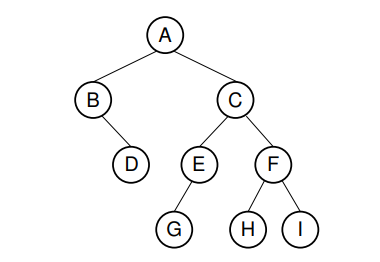
\includegraphics[scale = 0.8]{Capitoli/Alberi Binari/Esempi/Albero.png}
    
\end{center}
\textbf{in questa immagine abbiamo la rappresentazione di un albero binario}
\subsection{Profondità(Depth) e Altezza(Height)}
\begin{itemize}
    \item La \textbf{profondità} è la lunghezza del \textbf{path} da un nodo \textbf{M} a un nodo \textbf{N}. Tutti i nodi a \textbf{profondità d} risiedono al \textbf{livello d}
    \item \textbf{L'altezza è}: Partendo da un nodo \textbf{N} l'altezza è il numero di \textbf{archi} che devo attraversare per arrivare a una foglia(nodo più in profondità) quindi possiamo dire che l'altezza è \textbf{Depth}. il percorso valido verso le foglie è quello più lungo.
    \item la differenza tra \textbf{Depth} e \textbf{l'altezza} che sono inverse, scendendo \textbf{Depth} aumenta invece \textbf{l'altezza} diminuisce 
    \item il percorso valido verso le foglie è quello più lungo.
    \item Nel caso di un albero con un solo nodo allora si ha che la \textbf{Depth} e \textbf{l'altezza} sarà zero
    \item \textbf{P.S. :} La prof considera l'altezza come profondità + 1
\end{itemize}

\subsection{Nodi interni e foglie}
\begin{itemize}
    \item \textbf{Un nodo interno} è un nodo che ha almeno un figlio
    \item \textbf{Una foglia (leaf)} è un nodo senza figli
\end{itemize}
\subsection{Albero binario pieno}
\begin{itemize}
    \item Un albero è pieno quando per una certa altezza \textbf{h} ha il \textbf{numero massimo di nodi}, quindi ogni nodo interno ha sempre due figli.
\end{itemize}
\begin{center}
    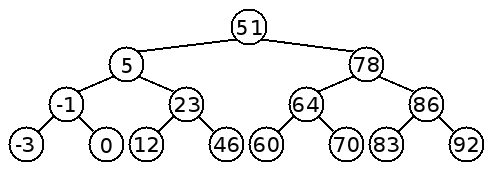
\includegraphics[scale = 0.6]{Capitoli/Alberi Binari/Esempi/AlberoPieno.png}
\end{center}
\newpage
\subsection{Albero binario completo}
\textbf{Un albero è detto completo se rispetta queste tre proprietà:}
\begin{enumerate}
    \item è un \textbf{albero binario}
    \item \textbf{le foglie} si trovano ad \textcolor{blue}{\textbf{altezza $h$ o $h-1$}}
    \item \textbf{al più un nodo} \textbf{\textcolor{blue}{interno}} può avere \textbf{meno di due figli}
\end{enumerate}
\begin{center}
    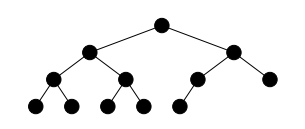
\includegraphics[scale = 0.8]{Capitoli/Alberi Binari/Esempi/alberocompleto.png}
\end{center}
\begin{tcolorbox}
    \textbf{\textcolor{blue}{NB:}} In questo corso per convenzione riempiamo un albero completo mettendo le foglie da \textbf{sinistra} verso \textbf{destra} in questo modo abbiamo la certezza che \textbf{tutti i livelli} siano pieni \textbf{eccetto} l'ultimo \textbf{livello} che può anche non essere pieno. L'albero di sopra rispetta questa proprietà.
\end{tcolorbox}

\subsection{Alberi binari Teoremi}
\textbf{un problema dei alberi binari} e che non c'è nessun vincolo di come io \textbf{posso posizionare} i miei dati, quindi può accadere che si crei una \textbf{catena}. In una struttura in cui i \textbf{dati sono solo} conservati nelle \textbf{foglie} questo potrebbe essere un grande problema poiché consuma molto spazio.
\begin{center}
    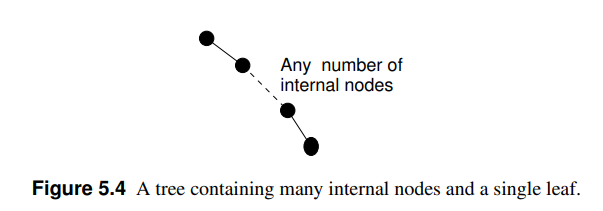
\includegraphics[scale = 0.6]{Capitoli/Alberi Binari/Esempi/catena.png}
\end{center}
\textbf{Per ovviare a questo problema ci sono molte altre famiglie di alberi binari come i alberi binari pieni un teorema molto importante ci dice:}
\subsubsection{Teorema: numero massimo di foglie in un albero pieno}
\textbf{\textcolor{blue}{Enunciato:}}\newline
\textit{Il numero di foglie in un albero pieno è uguale al numero di nodi interni più uno}\newline\newline
\newpage
\textbf{\textcolor{blue}{Dimostrazione:}}
\begin{itemize}
    \item Il teorema sarà dimostrato per induzione
    \item  \textbf{Caso base:} Per un albero altezza zero ($h = 0$) abbiamo che c'è solo una sola foglia, quindi i nodi interni sono: zero più uno è uguale a uno ($0+1 = 1$). Invece per altezza uno ($h = 1$) avrò un nodo interno , quindi uno più uno è uguale a 2 ($1+1 =2$), anche questa volta ci troviamo poiché essendo un albero pieno avremo due figli per l'unico nodo interno \textbf{(ovviamente un l'ipotesi è che stiamo lavorando su un albero binario pieno)}
    \item quindi osserviamo che sia per $h=0$ e $h = 1$ le nostra formula per calcolare le foglie è corretta cioè numero di nodi interni $n + 1$
    \item  \textbf{Ipotesi induttiva:} Ipotizziamo che ogni albero binario pieno $T$ abbia $n-1$ nodi interni e $n$ foglie.
    \item  \textbf{Passo induttivo:}
    Prendiamo un albero $T$ con $n$ nodi interni e prendiamo uno dei suoi nodi interni, lo chiamiamo $I$. Successivamente togliamo a questo nodo interno $I$ i due figli rendendolo cosi foglia. cosi facendo avremo un \textbf{sotto albero} $T'$ con $n-1$ nodi interni. Ora se prediamo $T'$ per la nostra ipotesi induttiva sappiamo che $T'$ ha $n$ foglie poiché ha $n-1$ nodi interni, se aggiungessimo a $T'$ le foglie che abbiamo tolto a $I$  cosa succederebbe? Avremo $T'$ con $n+2$ foglie, dobbiamo però toglierne una poiché la foglia a cui furono sottratti i figli ora è padre(non togliamo la foglia fisicamente ma solo dal conteggio), cosi avremo $n$ nodi interni e $n+1$ foglie. Abbiamo cosi dimostrato che anche aggiungendo due foglie(questo perché deve rimanere un albero binario pieno) avremo che il numero di foglie è il numero di nodi interni $+ 1$.
    
\end{itemize}
\subsubsection{Nodi pieni}
\begin{itemize}
    \item   \textbf{Un nodo è pieno} se ha due \textbf{figli} , se \textbf{non è pieno} è \textbf{foglia}(senza figli).
    \item  quindi ogni nodo o è \textbf{interno} o altrimenti è \textbf{foglia} non può avere un solo figlio.
\end{itemize}
\begin{center}
    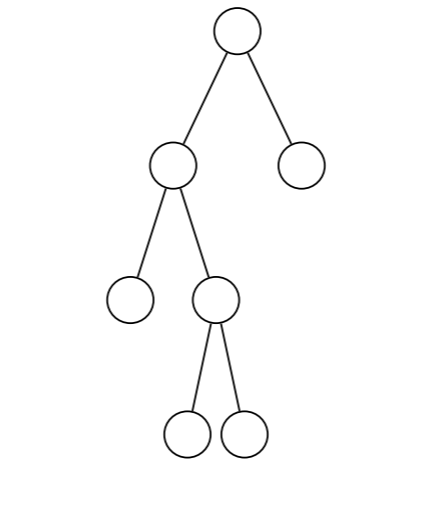
\includegraphics[scale = 0.3]{Capitoli/Alberi Binari/Esempi/NodiPieni.png}
\end{center}

\subsubsection{Definizione: alberi binari con figli non-vuoti e vuoti}
In questa immagine possiamo vedere che la figura (a) è un albero binario con la root con un foglio \textbf{sinistro} non vuoto, la figura (b)  è un albero binario con la root con un foglio \textbf{destro} non vuoto. Invece la (c)  è un albero binario con la root con il figlio \textbf{sinistro} vuoto, la (d)  è un albero binario con la root con il figlio \textbf{destro} vuoto
\begin{center}
    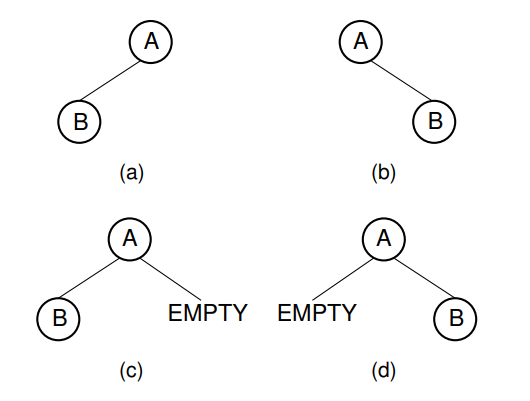
\includegraphics[scale = 0.5]{Capitoli/Alberi Binari/Esempi/Alberinonvuoti.png}
\end{center}
\subsubsection{Teorema: quanti sotto alberi vuoti ha un albero binario}
\textbf{\textcolor{blue}{Teorema}:} \textit{Il numero di  sotto alberi vuoti in un albero binario è il numero di nodi + 1}. \newline\newline
\textbf{\textcolor{blue}{Dimostrazione}:} Ogni albero binario $T$ ogni nodo ha due figli quindi per $n$ nodi un albero ha $2n$ figli dove $n$ è il numero di nodi. L'unico nodo senza parente è la root quindi possiamo dire che $n-1$ nodi hanno dei parenti.
sappiamo che $n-1$ nodi sono non vuoti. Togliendo al numero di figli totali il numero di nodi non vuoti ($n-1$) quindi otteniamo cosi $n+1$ che è il numero di sotto alberi vuoti poiché so che n-1 non sono vuoti

\newpage
\subsection{Modi di visitare L'albero}
\begin{itemize}
    \item \textbf{Traversal}: ogni processo per attraversare tutti i nodi in un certo ordine e che eseguono una specifica azione(es. stampare, sommare ecc.)
    \item Ogni \textbf{Traversal} che elenca ogni nodo \textbf{una sola} volta viene chiamata \textbf{Enumerazione(visita)}
    \item Gli \textbf{attraversamenti} possono seguire diversi ordini, tra cui:
    \begin{itemize}
        \item \textbf{\textcolor{blue}{Preorder}}: visito prima me stesso poi a sinistra e poi a destra.
        
        \item \textbf{\textcolor{blue}{Postorder}} : visito prima sinistra poi a destra e poi me stesso.
        
        \item \textbf{\textcolor{blue}{Inorder}}: visito prima sinistra poi me stesso e poi destra.
    \end{itemize}
    
    \begin{tcolorbox}[width=12cm, boxsep=10pt]
        \item \textbf{Esempio per contare nodi in un albero:}
        \lstinputlisting{Capitoli/Alberi Binari/Esempi/EsempioVisita.txt} 
    \end{tcolorbox}
\end{itemize} 
\subsection{Spazio richiesto per albero binario}
\begin{itemize}
    \subsubsection{Struttura}
    \item \textbf{Il nodo} deve contenere lo \textbf{spazio} per il dato e per i due \textbf{puntatori ai figli}
    \item \textbf{OverHead:} Il "overhead" per lo spazio di un albero si riferisce alla quantità di memoria aggiunta a quella utilizzata dai dati effettivi memorizzati nei nodi dell'albero.
    \item Quindi \textbf{l'overhead} è lo spazio richiesto per memorizzare tutto quello che non è il dato. quindi tutto quello che riguarda la struttura dati è \textbf{overhead}.
    
    \item  infatti \textbf{l'overhead} dipende da:
    \begin{itemize}
        \item in quale tipo di nodi memorizzo i dati (tutti, solo le foglie, . . . )
        \item se le foglie contengono comunque puntatori nulli
        \item se l’albero è a nodi pieni
    \end{itemize}
    \newpage
    \subsubsection{Spazio Richiesto}
    \item \textbf{Dato è piccolo}
    \begin{itemize}
        \item \textbf{\textcolor{blue}{Costo Totale:}} $n(2P + D)$ \newline\textbf{n} numero di nodi \textbf{P} sono i puntatori e \textbf{D} il dato
        \item \textbf{\textcolor{blue}{OverHead:}} $2nP$ senza il dato poiché è lo spazio richiesto in piu oltre al dato effettivo.
        \item \textbf{\textcolor{blue}{Percentuale di overhead:}} $2P/(2P + D)$ quindi se $P = D$ avrò il 2/3 di spazio che è \textbf{overhead}
    \end{itemize}
    \item \textbf{Se il dato è grande, nel nodo metto solo il puntatore}
    \item  Ho quindi tre puntatori, tutti di \textbf{overhead}:
    \begin{itemize}
        \item \textbf{\textcolor{blue}{Costo Totale:}} $n(3P + D)$ \newline\textbf{n} numero di nodi \textbf{P} sono i puntatori e \textbf{D} il dato
        \item \textbf{\textcolor{blue}{OverHead:}} $3nP$ senza il dato poiché è lo spazio richiesto in piu oltre al dato effettivo.
        \item \textbf{\textcolor{blue}{Percentuale di overhead:}} $3P/(3P + D)$ quindi se $P = D$ avrò il 3/4 di spazio che è \textbf{overhead}
    \end{itemize}

    \item \textbf{Se invece l'albero è pieno e non ho puntatori sulle foglie l'overhead è:}
    \begin{itemize}
        \item \textbf{\textcolor{blue}{Costo Totale:}} Avremo $2P + D$ per circa $n/2$ \textbf{nodi interni}.\newline Nelle foglie avremo $D$ per circa $n/2$ \textbf{foglie}. \newline\newline Quindi in totale avremo $\dfrac{n}{2}(2P+2D)$
        \item \textbf{\textcolor{blue}{OverHead:}} $\dfrac{n}{2}(2P)$
        \item \textbf{\textcolor{blue}{Percentuale di overhead:}} \newline\newline $\dfrac{\dfrac{n}{2}(2P)}{\dfrac{n}{2}(2P) + nD} = \dfrac{P}{P+D}$ 
        \item Se $D = P$ allora la percentuale di overhead è circa $1/2$
    \end{itemize}
\end{itemize}
\newpage
\textbf{\textcolor{blue}{Puntatori ai dati solo nelle foglie:}}
\begin{center}
    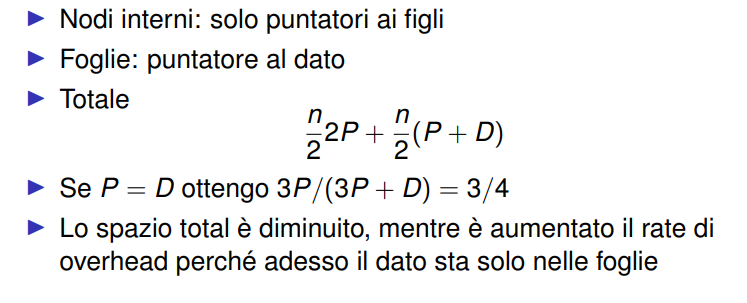
\includegraphics[scale = 0.7]{Capitoli/Alberi Binari/Esempi/DatoFigli.png}
\end{center}

\newpage
\subsection{Implementazione di un albero binario (Vettore)}
\begin{itemize}
    \item  Se conosciamo la struttura dell’albero, possiamo ridurre
    l’overhead legato ai puntatori.
    
    \item Se \textbf{l’albero binario è completo}, dato il numero di nodi \textbf{n} la
    sua struttura è unica.

    \item Questa \textbf{tecnica} funziona con i \textbf{alberi completi} poiché hanno un pattern ben preciso. Per funzionare questa tecnica ha bisogno che le foglie devono essere posizionate da \textbf{destra} verso \textbf{sinistra}.
    
    \item \textbf{Numero i nodi partendo dalla radice e scorrendo ciascun
    livello da sinistra verso destra in modo univoco}.
    
    \item \textbf{Questa numerazione mi dà la posizione all’interno
    dell’array:}

    \begin{itemize}
        \item \textcolor{blue}{\code{Parent(r)}} $= \left\lfloor \frac{r - 1}{2} \right\rfloor$ se $r \neq 0$
        \item \textcolor{blue}{\code{LeftChild(r)}} $= 2r + 1$ se $2r + 1 < n$
        \item \textcolor{blue}{\code{RightChild(r)}} $= 2r + 2$ se $2r + 2 < n$
        \item \textcolor{blue}{\code{LeftSibling(r)}}\textsuperscript{1} $= r - 1$ se $r$ è pari
        \item \textcolor{blue}{\code{RightSibling(r)}} $= r + 1$ se $r$ è dispari e $r + 1 < n$
    \end{itemize}
    \begin{center}
        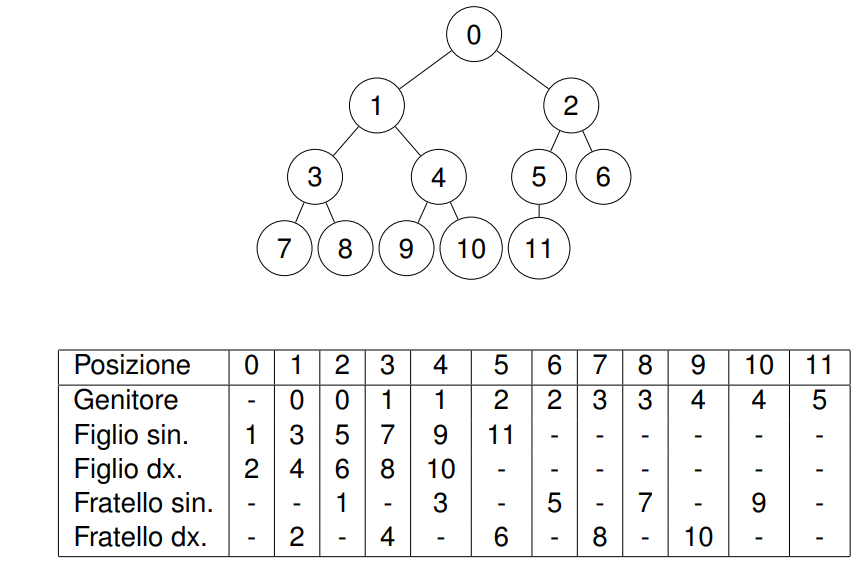
\includegraphics[scale = 0.6]{Capitoli/Alberi Binari/Esempi/AlberoFromArray.png}
    \end{center}
    \footnotetext[1]{Da il fratello Sinistro di $r$, se $r$ è il figlio destro LeftSibling(r) non restituisce nulla}
\end{itemize}
